%% Towards a Cartography of Datacentering
%% Research Policy 11th ECR Conference · 27 April 2026 · 14:27 BST
%% Tufte-inspired Beamer — pdflatex + lmodern (no xelatex required)

\documentclass[aspectratio=169,12pt]{beamer}

%% Fonts: Latin Modern serif (Tufte-style)
\usepackage{lmodern}
\usepackage[T1]{fontenc}
\usepackage[utf8]{inputenc}
\usefonttheme{serif}

%% Packages
\usepackage{booktabs}
\usepackage{tabularx}
\usepackage{array}
\usepackage{tikz}
\usepackage{graphicx}
\usepackage{xcolor}
\usepackage{microtype}
\usepackage{textcomp}
\usetikzlibrary{arrows.meta,positioning,fit}

%% Tufte colour palette
\definecolor{tufteText}{HTML}{222222}
\definecolor{tufteRule}{HTML}{888888}
\definecolor{tufteAccent}{HTML}{B85C00}   %% warm orange
\definecolor{tufteLight}{HTML}{F5F0EA}    %% warm off-white for backgrounds
\definecolor{tufteMid}{HTML}{CCCCCC}

%% Minimal theme
\usetheme{default}
\useinnertheme{default}
\useoutertheme{default}
\setbeamertemplate{navigation symbols}{}

%% Colours
\setbeamercolor{normal text}{fg=tufteText,bg=white}
\setbeamercolor{structure}{fg=tufteAccent}
\setbeamercolor{alerted text}{fg=tufteAccent}
\setbeamercolor{example text}{fg=tufteRule}
\setbeamercolor{itemize item}{fg=tufteRule}
\setbeamercolor{itemize subitem}{fg=tufteRule}
\setbeamercolor{enumerate item}{fg=tufteAccent}
\setbeamercolor{frametitle}{fg=tufteText,bg=white}
\setbeamercolor{title}{fg=tufteText}
\setbeamercolor{subtitle}{fg=tufteRule}
\setbeamercolor{author}{fg=tufteText}
\setbeamercolor{date}{fg=tufteRule}
\setbeamercolor{footline}{fg=tufteRule}
\setbeamercolor{block title}{fg=tufteAccent,bg=white}
\setbeamercolor{block body}{fg=tufteText,bg=tufteLight}

%% Fonts
\setbeamerfont{frametitle}{series=\bfseries,size=\large}
\setbeamerfont{title}{size=\LARGE,series=\bfseries}
\setbeamerfont{subtitle}{size=\normalsize,shape=\itshape,series=\mdseries}
\setbeamerfont{author}{size=\normalsize,series=\mdseries}
\setbeamerfont{date}{size=\small,series=\mdseries}
\setbeamerfont{footline}{size=\tiny}
\setbeamerfont{itemize/enumerate body}{size=\normalsize}
\setbeamerfont{itemize/enumerate subbody}{size=\small}

%% Frame title with thin rule
\setbeamertemplate{frametitle}{%
  \vspace{0.5em}%
  \insertframetitle\par%
  \vspace{0.15em}%
  \textcolor{tufteRule}{\rule{\textwidth}{0.4pt}}%
  \vspace{0.2em}%
}

%% Quiet bullets
\setbeamertemplate{itemize item}{\textcolor{tufteRule}{\small$\bullet$}}
\setbeamertemplate{itemize subitem}{\textcolor{tufteRule}{\scriptsize$\circ$}}
\setbeamertemplate{enumerate item}{\textcolor{tufteAccent}{\insertenumlabel.}}

%% Footer: slide number only
\setbeamertemplate{footline}{%
  \hfill\textcolor{tufteRule}{\tiny\insertframenumber}\hspace{1.2em}\vspace{0.6em}%
}

%% Generous margins
\setbeamersize{text margin left=1.6em, text margin right=1.6em}
\hfuzz=26pt

%% Table defaults
\renewcommand{\arraystretch}{1.25}

%% ===================================================================
\title{Towards a Cartography of Datacentering}
\subtitle{A Multimodal Research Agenda for Innovation Studies}
\author{Babajide Alamu Owoyele}
\institute{DRIFT, Erasmus University Rotterdam\\
           Radboud University Donders Institute}
\date{Research Policy 11th ECR Conference · 27 April 2026}

\setbeameroption{hide notes}

\begin{document}

%% -------------------------------------------------------------------
%% SLIDE 1 — Title  (0:15)
\begin{frame}[plain]
\vspace{2.5em}
{\usebeamerfont{title}\usebeamercolor[fg]{title}\inserttitle\par}
\vspace{0.4em}
{\usebeamerfont{subtitle}\usebeamercolor[fg]{subtitle}\insertsubtitle\par}
\vspace{1.2em}
\textcolor{tufteRule}{\rule{0.4\textwidth}{0.4pt}}\par
\vspace{0.5em}
{\usebeamerfont{author}\insertauthor\par}
\vspace{0.15em}
{\footnotesize\textcolor{tufteRule}\insertinstitute\par}
\vspace{0.4em}
{\usebeamerfont{date}\usebeamercolor[fg]{date}\insertdate\par}
\note{I'm proposing a methodological cartography for studying data-center infrastructure as a contested innovation arena. Ten minutes.}
\end{frame}

%% -------------------------------------------------------------------
%% SLIDE 2 — The Empirical Moment  (0:45)
\begin{frame}{The Empirical Moment}
\begin{columns}[T]
\begin{column}{0.48\textwidth}
  \begin{tabular}{@{}lr@{}}
    \toprule
    \textbf{Metric} & \textbf{Value} \\
    \midrule
    Hyperscaler capex 2026  & \textbf{\$750B} \\
    DC electricity 2025     & 485 TWh (+17\%) \\
    AI-specific growth      & +50\% YoY \\
    Hyperscaler share 2031  & 67\% of all DC \\
    \bottomrule
  \end{tabular}
  \vspace{0.8em}

  \footnotesize\textcolor{tufteRule}{%
  CreditSights Feb 2026; IEA Energy \& AI April 2026;\\
  Synergy Research Group}
\end{column}
\begin{column}{0.48\textwidth}
  \vspace{0.3em}
  \large\textit{``The largest concentrated\\
  infrastructure build of our\\
  lifetimes — happening now.''}

  \vspace{0.8em}
  \normalsize
  Not a future scenario.\\
  Not a policy proposal.\\[0.3em]
  \alert{An arena in formation.}
\end{column}
\end{columns}
\note{Lead with the dollar number. Don't read the table — point at it. Hyperscaler capex is the largest concentrated infrastructure build of our lifetimes, and it's happening in three years.}
\end{frame}

%% -------------------------------------------------------------------
%% SLIDE 3 — Why Now? The Contested Arena  (0:45)
\begin{frame}{Why Now? The Contested Arena}
\begin{columns}[T]
\begin{column}{0.52\textwidth}
  \begin{itemize}\setlength\itemsep{0.5em}
    \item \textbf{Stargate:} \$500B / $\sim$7 GW committed;
          fragmented (OpenAI, Oracle, SoftBank)
    \item \textbf{PJM electricity:} capacity prices \alert{+833\%} in one year
    \item \textbf{Maine:} statewide moratorium, April 2026
    \item \textbf{Loudoun County:} eliminates by-right DC, March 2025
    \item \textbf{DeepSeek V4-Pro:} re-opens Jevons paradox debate
  \end{itemize}
\end{column}
\begin{column}{0.44\textwidth}
  \vspace{0.5em}
  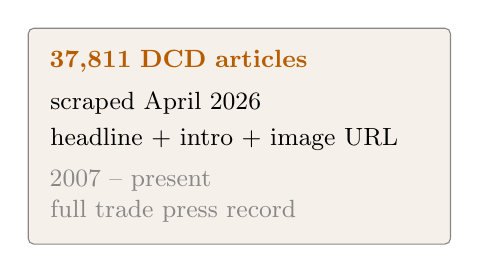
\begin{tikzpicture}[font=\small]
    \node[draw=tufteRule,rounded corners=2pt,
          inner sep=8pt,text width=4.8cm,
          fill=tufteLight,align=left] {
      \textcolor{tufteAccent}{\textbf{37,811 DCD articles}}\\[4pt]
      scraped April 2026\\[2pt]
      headline + intro + image URL\\[4pt]
      \textcolor{tufteRule}{\small 2007 -- present}\\
      \textcolor{tufteRule}{\small full trade press record}
    };
  \end{tikzpicture}
  \vspace{0.4em}

  \footnotesize\textit{The arena is visible in the\\
  trade press before it appears\\
  in the academic literature.}
\end{column}
\end{columns}
\note{Five bullets, two seconds each. The point is the arena is contested right now. Maine moratorium is April 2026 — last month. This is not a stable industry settling — it's a contested arena in formation.}
\end{frame}

%% -------------------------------------------------------------------
%% SLIDE 4 — The Gap  (0:45)
\begin{frame}{The Gap in Innovation Studies}
\begin{columns}[T]
\begin{column}{0.48\textwidth}
  \small\textbf{RP canon covers:}\\[0.4em]
  \footnotesize
  Platforms (Gawer 2014)\\
  GPTs and productivity (Brynjolfsson)\\
  Sectoral systems (Malerba)\\
  Transitions (Geels)\\[0.6em]

  \small\textbf{Critical DC studies exists:}\\[0.4em]
  \footnotesize
  \textit{Big Data \& Society}, \textit{Convergence}\\
  (Edwards et al.\ 2025; Monstadt 2025)\\
  — but outside RP's intellectual canon
\end{column}
\begin{column}{0.48\textwidth}
  \vspace{0.2em}
  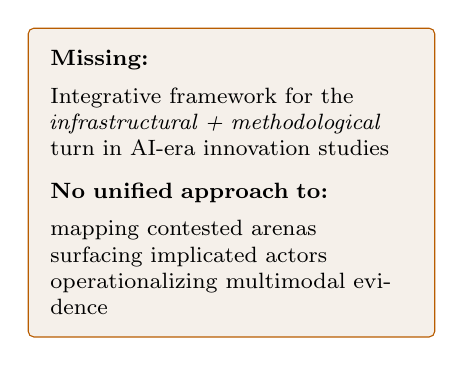
\begin{tikzpicture}[font=\footnotesize]
    \node[draw=tufteAccent,rounded corners=2pt,
          inner sep=8pt,text width=4.6cm,
          fill=tufteLight] {
      \textbf{Missing:}\\[4pt]
      Integrative framework for the\\
      \textit{infrastructural + methodological}\\
      turn in AI-era innovation studies\\[6pt]
      \textbf{No unified approach to:}\\[4pt]
      mapping contested arenas\\
      surfacing implicated actors\\
      operationalizing multimodal evidence
    };
  \end{tikzpicture}
\end{column}
\end{columns}
\note{RP has the tools — arenas, transitions, sectoral systems. Critical data-center studies exists in BD&S and Convergence, but outside RP. Nobody has bridged them. That's the gap.}
\end{frame}

%% -------------------------------------------------------------------
%% SLIDE 5 — Theory Layer 1: Arenas  (0:50)
\begin{frame}{Theory Layer 1: Arenas of Development}
\begin{columns}[T]
\begin{column}{0.52\textwidth}
  \textbf{Jørgensen (2012) — \textit{Research Policy}}\\[0.3em]
  \footnotesize
  ``Mapping and navigating transitions: The MLP compared with arenas of development''\\[0.6em]

  \small\textbf{Key move: flat ontology}\\[0.3em]
  \footnotesize
  Start from \textit{actor constellations}\\
  and their collective engagement,\\
  not pre-classified structural tiers.\\[0.4em]
  \textbf{Negotiation} is the fundamental process.\\[0.4em]
  Allows political, social, environmental\\
  spheres simultaneously.
\end{column}
\begin{column}{0.44\textwidth}
  \vspace{0.4em}
  \footnotesize\textbf{For datacentering:}\\[0.3em]
  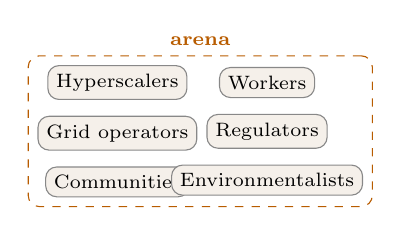
\begin{tikzpicture}[font=\scriptsize,
    node distance=0.2cm,
    actor/.style={draw=tufteRule,rounded corners,
                  inner sep=3pt,fill=tufteLight}]
    \node[actor] (h)  {Hyperscalers};
    \node[actor,below=of h] (g) {Grid operators};
    \node[actor,below=of g] (c) {Communities};
    \node[actor,right=0.4cm of h] (w)  {Workers};
    \node[actor,below=of w] (r)  {Regulators};
    \node[actor,below=of r] (e)  {Environmentalists};
    \node[draw=tufteAccent,dashed,rounded corners,
          fit=(h)(g)(c)(w)(r)(e),
          label=above:{\textcolor{tufteAccent}{\textbf{arena}}}]{};
  \end{tikzpicture}
  \vspace{0.3em}

  \footnotesize
  Co-constitutive — not hierarchically ordered.
\end{column}
\end{columns}
\note{Arenas, not levels. Flat ontology. Negotiation is the process. Hyperscalers, grid operators, communities, workers, regulators are co-constitutive — not hierarchically ordered. Jørgensen is in RP — this is your canon, not an import.}
\end{frame}

%% -------------------------------------------------------------------
%% SLIDE 6 — Theory Layer 2: Situational Analysis  (0:50)
\begin{frame}{Theory Layer 2: Situational Analysis}
\begin{columns}[T]
\begin{column}{0.52\textwidth}
  \textbf{Clarke (2005) — STS / Grounded Theory}\\[0.3em]
  \footnotesize
  Extends Strauss with three kinds of maps:\\[0.3em]
  \begin{enumerate}\setlength\itemsep{0.2em}
    \item Situational maps (all human/nonhuman elements)
    \item Social worlds / arenas maps
    \item Positional maps
  \end{enumerate}
  \vspace{0.4em}
  \small\textbf{Key innovation: implicated actors}\\[0.3em]
  \footnotesize
  (1) Silenced / made invisible by power\\
  (2) Discursively constructed but absent
\end{column}
\begin{column}{0.44\textwidth}
  \vspace{0.3em}
  \footnotesize\textbf{For datacentering:}\\[0.4em]
  \begin{tabular}{@{}ll@{}}
    \textit{Decided by:} & boards, planners \\[0.2em]
    \textit{Silenced:}   & communities,\\
                         & visa workers \\[0.2em]
    \textit{Invoked:}    & ``the consumer''\\
                         & ``future generations'' \\
  \end{tabular}
  \vspace{0.5em}

  \footnotesize\alert{Who is excluded from\\
  the negotiation?\\
  Who is invoked but absent?}
\end{column}
\end{columns}
\note{Three maps. The key innovation is implicated actors — silenced AND discursively constructed. Who is excluded from the negotiation? Communities, visa workers. Who is invoked but absent? The consumer, future generations. Clarke gives us a method for making this systematic.}
\end{frame}

%% -------------------------------------------------------------------
%% SLIDE 7 — Theory Layer 3: Marres + CITC  (0:50)
\begin{frame}{Theory Layer 3: Issue Mapping + CITC}
\begin{columns}[T]
\begin{column}{0.50\textwidth}
  \textbf{Marres (2015)}\\
  \footnotesize
  Issue mapping via digital traces:\\
  hyperlinks, hashtags, discourse networks.\\
  \textit{Affirmative} approach: traces as\\
  empirical window into issue formation.\\[0.5em]

  \textbf{Berente, Seidel \& Safadi (2019)\\
  Miranda et al.\ (2022) — CITC}\\[0.2em]
  \footnotesize
  Computationally Intensive Theory Construction:\\
  sampling $\to$ synchronic $\to$ diachronic\\
  $\to$ \textbf{lexical framing}\\[0.3em]
  Patterns become contributions \textit{only}\\
  once situated in scholarly discourse.
\end{column}
\begin{column}{0.46\textwidth}
  \vspace{0.5em}
  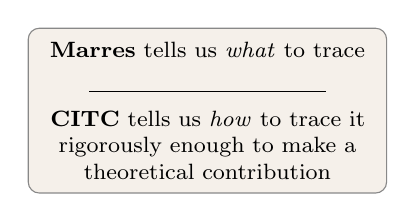
\begin{tikzpicture}[font=\footnotesize,node distance=0.25cm]
    \node[draw=tufteRule,rounded corners,fill=tufteLight,
          inner sep=5pt,text width=4.2cm,align=center] {
      \textbf{Marres} tells us \textit{what} to trace\\[3pt]
      \rule{3cm}{0.3pt}\\[3pt]
      \textbf{CITC} tells us \textit{how} to trace it\\
      rigorously enough to make a\\
      theoretical contribution
    };
  \end{tikzpicture}
  \vspace{0.4em}

  \footnotesize\textcolor{tufteRule}{Prevents atheoretical\\
  pattern-mining.\\
  The test for RP.}
\end{column}
\end{columns}
\note{DO NOT READ THE FOUR STEPS. One sentence to land: Marres tells us what to trace. CITC tells us how to trace it rigorously enough to make a theoretical contribution. If time, mention lexical framing as the discipline that prevents atheoretical pattern-mining.}
\end{frame}

%% -------------------------------------------------------------------
%% SLIDE 8 — Methods: Operationalizing  (1:15)
\begin{frame}[shrink=5]{Operationalizing: Multimodal Data Sources}
\vspace{0.1em}
{\footnotesize
\begin{tabularx}{\textwidth}{@{}lXX@{}}
  \toprule
  \textbf{Modality} & \textbf{Source / method} & \textbf{Output} \\
  \midrule
  \textbf{Text} &
    DCD news corpus (37,552 articles, 2008--2026);\newline
    1,190 contestation events; topic modelling;\newline
    registerial analysis (Matthiessen 2015) &
    Topic distributions + verb process types\\
    & \textcolor{tufteRule}{\scriptsize + GLiNER NER · BERTopic · CITC cycle} & \\
  \addlinespace[3pt]
  \textbf{Image} &
    Satellite (Sentinel-2, Landsat LST);\newline
    DCD article images; corporate photography &
    Land conversion maps;\newline visual register index (CLIP + BERTopic)\\
  \addlinespace[3pt]
  \textbf{Graph} &
    Hyperlink networks; ownership (SEC EDGAR, REIT filings);\newline
    urban embeddedness (city2graph + Overture Maps) &
    Arena actor maps;\newline governance counterparty analysis\\
  \addlinespace[3pt]
  \textbf{Structured} &
    Crunchbase / 10-Ks; planning records &
    Funding flows;\newline capex + geography diffusion\\
  \bottomrule
\end{tabularx}}
\vspace{0.3em}
\footnotesize\textcolor{tufteRule}{Each modality runs through the CITC cycle. This is operationalized, not theoretical.}
\note{Four data sources, four expected outputs. Don't read the slide. Point at each row, name it, name what it produces. Close with: each modality runs through the CITC cycle. This is operationalized, not theoretical.}
\end{frame}

%% -------------------------------------------------------------------
%% SLIDE 9 — DCD corpus: what the data shows
\begin{frame}{The Arena in Data: 37,552 Articles, 1,190 Contestation Events}
\begin{columns}[T]
\begin{column}{0.50\textwidth}
  \includegraphics[width=\textwidth,height=0.65\textheight,keepaspectratio]%
    {../figures/dcd_eda_timeline}
\end{column}
\begin{column}{0.46\textwidth}
  \includegraphics[width=\textwidth,height=0.65\textheight,keepaspectratio]%
    {../figures/dcd_eda_geography}
\end{column}
\end{columns}
\vspace{0.2em}
\footnotesize\textcolor{tufteRule}{%
  Peak contestation year: 2025.
  Top triggers: legal/court, planning refusal, community opposition, moratorium.
  \textbf{Analysis on headlines + intro text only} (first 1--2 sentences).
  Full article text via screenshot/OCR pipeline: more coming.}
\note{This is from the real corpus — 37,552 articles, 2008 to 2026. Peak contestation in 2025. Maine statewide moratorium is in this data. The arena isn't a hypothesis — it's visible in the trade press record.}
\end{frame}

%% -------------------------------------------------------------------
%% SLIDE 10 — Register finding
\begin{frame}{What the Verb Register Shows}
\begin{columns}[T]
\begin{column}{0.50\textwidth}
  \includegraphics[width=\textwidth,height=0.65\textheight,keepaspectratio]%
    {../figures/register_contrast}
\end{column}
\begin{column}{0.46\textwidth}
  \vspace{0.5em}
  \small\textbf{Key shift (Matthiessen 2015)}\\[0.4em]
  \footnotesize
  \begin{tabular}{@{}lrr@{}}
    \toprule
    Process type & Contest & Non \\
    \midrule
    Behavioral   & 23.1\% & 1.6\% \\
    Enabling     & 16.5\% & 3.1\% \\
    Material     & 33.7\% & 66.8\% \\
    \bottomrule
  \end{tabular}
  \vspace{0.5em}

  \footnotesize
  \textit{Doing} $\to$ \textit{enabling/exploring}\\[0.3em]
  The arena shifts from\\
  building to governing\\
  and contesting.\\[0.4em]
  \alert{This is the governance gap\\
  in its linguistic signature.}\\[0.4em]
  \textcolor{tufteRule}{\scriptsize Headlines + intros only.\\
  Full articles: more coming.}
\end{column}
\end{columns}
\note{The register shift is the governance gap made linguistic. Contestation coverage has 21.5\% more behavioral verbs and 13.4\% more enabling verbs. Material verbs drop 33\%. The arena has shifted from building to governing. Headlines and intro text only. Full article text comes through screenshot/OCR pipeline.}
\end{frame}

%% -------------------------------------------------------------------
%% SLIDE 11 (renumbered) — Research Agenda 1: Regional Innovation Systems  (0:50)
\begin{frame}{Research Agenda 1: Regional Innovation Systems}
\small\textbf{Central question:} How do hyperscale data-center clusters reshape
local productivity, labour markets, energy regimes, and property relations?\\[0.5em]
\begin{columns}[T]
\begin{column}{0.48\textwidth}
  \footnotesize
  \begin{tabular}{@{}ll@{}}
    \textbf{Cases:}    & Loudoun (US), Lul\r{e}å (SE) \\
                       & Dublin (IE), Hyderabad (IN) \\[0.3em]
    \textbf{Metrics:}  & Employment volatility \\
                       & Electricity price shocks \\
                       & Tax dependence \\
                       & Community displacement \\
  \end{tabular}
\end{column}
\begin{column}{0.48\textwidth}
  \footnotesize
  \textbf{From DCD corpus:}\\[0.3em]
  News framing shift:\\
  pro-growth $\to$ environmental concern\\[0.3em]
  City2graph:\\
  residential adjacency + power density\\[0.3em]
  \alert{Amsterdam: moratorium $<$1yr after\\
  signal onset.\\
  Virginia: comparable signal, no response.}
\end{column}
\end{columns}
\note{Question, cases, metrics, expected figures. Don't dwell. This is a program the cartography enables.}
\end{frame}

%% -------------------------------------------------------------------
%% SLIDE 10 — Research Agenda 2: Sectoral Transformation  (0:50)
\begin{frame}{Research Agenda 2: Sectoral Transformation}
\small\textbf{Central question:} How does hyperscaler vertical integration reshape
sectoral innovation systems, especially in AI-using industries?\\[0.5em]
\begin{columns}[T]
\begin{column}{0.48\textwidth}
  \footnotesize
  \textbf{Mechanism:}\\
  AWS, Google, Meta, Microsoft\\
  control compute + models + stacks\\[0.4em]
  \textbf{Effect:}\\
  Changed startup access\\
  New forms of lock-in\\
  Shifted innovation incentives
\end{column}
\begin{column}{0.48\textwidth}
  \footnotesize
  \textbf{Evidence:}\\
  Hyperlink networks of startup funding\\
  (hyperscaler-mediated vs.\ traditional VC)\\[0.3em]
  Crunchbase exit patterns\\[0.3em]
  News coverage of\\
  ``platform dependency'' clusters
\end{column}
\end{columns}
\note{Same structure: question, mechanism, evidence. Don't dwell.}
\end{frame}

%% -------------------------------------------------------------------
%% SLIDE 11 — Research Agenda 3: Policy Sovereignty  (0:50)
\begin{frame}{Research Agenda 3: Policy Sovereignty \& Energy}
\small\textbf{Central question:} What policy mix sustains sovereign compute
capacity without fossil-fuel dependence or geopolitical lock-in?\\[0.5em]
\begin{columns}[T]
\begin{column}{0.48\textwidth}
  \footnotesize
  \textbf{Cases:}\\
  UK AI Growth Zones\\
  EU AI Factories\\
  France \texteuro 109B investment\\
  Saudi HUMAIN · UAE Stargate\\[0.4em]
  \textbf{Instruments:}\\
  Grid access, renewables mandates,\\
  labour standards, tax incentives
\end{column}
\begin{column}{0.48\textwidth}
  \footnotesize
  \textbf{Evidence:}\\
  Policy document discourse SNA\\[0.3em]
  Capital flows to sovereign projects\\[0.3em]
  Regulatory filing timelines\\[0.3em]
  \alert{Policy innovation diffusion curves}
\end{column}
\end{columns}
\note{Same structure. Don't dwell. Three research agendas total — each is a program, not just a paper.}
\end{frame}

%% -------------------------------------------------------------------
%% SLIDE 12 — What This Enables  (0:30)
\begin{frame}{What This Enables: Methodological Innovation}
\begin{columns}[T]
\begin{column}{0.52\textwidth}
  \begin{itemize}\setlength\itemsep{0.4em}
    \item \textbf{Empirical cartography:} contested infrastructure transitions
          made visually traceable and empirically accountable
    \item \textbf{Multi-arena mapping:} surfaces who is included, excluded,
          silenced, or discursively constructed
    \item \textbf{Toolkit for RP:} replicable for energy, telecom, rare earths,
          supply chains — any contested infrastructure transition
  \end{itemize}
\end{column}
\begin{column}{0.44\textwidth}
  \begin{itemize}\setlength\itemsep{0.4em}
    \item \textbf{Bridge STS $\leftrightarrow$ Innovation:} critical
          infrastructure scholarship $\to$ RP policy canon
    \item \textbf{Open science:} methodological infrastructure for multimodal
          evidence synthesis across disciplines
  \end{itemize}
  \vspace{0.5em}
  \footnotesize\textcolor{tufteRule}{%
  \texttt{github.com/babajideowoyele/}\\\texttt{datacentering-cartography}}
\end{column}
\end{columns}
\note{Five bullets in 30 seconds. The toolkit move: this isn't only datacentering. It applies to energy, telecom, rare earths, supply chains — any contested infrastructure transition.}
\end{frame}

%% -------------------------------------------------------------------
%% SLIDE 13 (CLOSING PROMPT)  (0:15)
\begin{frame}[plain]
\vspace{2.5em}
{\large\itshape
What would innovation studies look like if we treated\\[0.4em]
data infrastructure buildout — both as physical facilities\\[0.4em]
and as research infrastructure — as\\[0.6em]}
{\Large\textbf{\alert{foundational} rather than peripheral?}}\\[1.2em]
\textcolor{tufteRule}{\rule{0.5\textwidth}{0.4pt}}\\[0.6em]
{\normalsize A cartography of datacentering is one answer.}\\[0.3em]
{\small\textit{What are others?}}
\note{Read the question slowly. Hold the silence for one beat. Then: What are others?}
\end{frame}

%% ===================================================================
%% BACKUP — Loudoun situational map  (Q&A)
%% ===================================================================
\appendix

\begin{frame}[noframenumbering]{Backup: Loudoun County Arena (Situational Map)}
\begin{columns}[T]
\begin{column}{0.50\textwidth}
  \small\textbf{Actors}\\[0.3em]
  \footnotesize
  \begin{tabular}{@{}ll@{}}
    Hyperscalers   & Amazon AWS, Google, Meta \\
    Energy         & Dominion Energy \\
    Planning       & Loudoun County Board \\
    Opposition     & Sierra Club, Piedmont EC \\
    Labour         & visa workers + local \\
  \end{tabular}
  \vspace{0.4em}

  \small\textbf{Nonhuman actants}\\[0.2em]
  \footnotesize
  Electricity grid · hyperscale facilities\\
  Zoning laws · satellite time-series
\end{column}
\begin{column}{0.46\textwidth}
  \small\textbf{Discourses in corpus}\\[0.3em]
  \footnotesize
  ``Tech economic engine''\\
  ``Environmental burden''\\
  ``Worker precarity''\\[0.5em]

  \small\textbf{Registerial signal}\\[0.3em]
  \footnotesize
  Verb register 2019--2024:\\
  material $\uparrow$ enabling $\uparrow$\\
  relational $\downarrow$\\[0.3em]
  \alert{Action displacing description}\\
  = arena in contestation
\end{column}
\end{columns}
\end{frame}

\begin{frame}[noframenumbering]{Q: Isn't this just STS dressed up as innovation studies?}
\footnotesize
\textbf{Live:} ``Fair concern — I'm using Jørgensen and Marres specifically
because they bridge to RP and \textit{ST\&HV}, not importing critical theory wholesale.''\\[0.6em]

\textbf{The methodological spine:}\\
CITC (Berente, Seidel \& Safadi 2019; Miranda et al.\ 2022) comes from
\textit{MIS Quarterly} and \textit{ISR} — not from STS.\\[0.6em]

The agenda is testable, not hermeneutic.\\[0.4em]
Slide 13 makes the RP positioning explicit.
\end{frame}

\begin{frame}[noframenumbering]{Q: Where's the empirical contribution?}
\footnotesize
\textbf{Live:} ``The ECR paper is the agenda. The Loudoun pilot is the first
empirical instantiation — I can speak to that.''\\[0.6em]

\textbf{Deliberate sequencing:} the agenda paper exists to make the
methodology citable \textit{before} the empirical papers, so reviewers of
those papers have a coherent framework to reference.\\[0.6em]

\textbf{From 37,811 DCD articles:}\\[0.3em]
\begin{tabular}{@{}lll@{}}
  \toprule
  \textbf{Analysis} & \textbf{Status} & \textbf{Finding} \\
  \midrule
  EDA geography     & Complete  & US/Europe split visible at N=37K \\
  Register analysis & Running   & Verb types by city \\
  BERTopic          & Queued    & Topic clusters on full corpus \\
  city2graph        & Seed run  & 3 cities, scales with NER \\
  \bottomrule
\end{tabular}
\end{frame}

\begin{frame}[noframenumbering]{Q: Why CITC and not computational social science more broadly?}
\footnotesize
\textbf{Live:} ``Because CITC's lexical-framing requirement is what makes
the output theoretical, not just descriptive. That's the test for RP.''\\[0.6em]

CITC explicitly distinguishes patterns from contributions.\\[0.4em]
That's the discipline that protects against the most common reviewer
objection to digital-trace work:\\[0.4em]
\begin{quote}
  ``This is interesting, but what's the theoretical contribution?''
\end{quote}
\end{frame}

\begin{frame}[noframenumbering]{Q: Why Loudoun, Luleå, Dublin, Hyderabad?}
\footnotesize
\textbf{Variation on three dimensions:}\\[0.4em]
\begin{tabular}{@{}llll@{}}
  \toprule
  \textbf{Case} & \textbf{Regulatory regime} & \textbf{Energy mix} & \textbf{Industrial trajectory} \\
  \midrule
  Loudoun    & Common law / NIMBY  & Gas + solar       & Mature US cluster \\
  Lule\r{a}  & Swedish planning    & 98\% hydro        & Renewable-led \\
  Dublin     & Irish planning      & Mixed, constrained & FDI platform \\
  Hyderabad  & Indian regulatory   & Mixed, expanding  & Emerging South Asian hub \\
  \bottomrule
\end{tabular}
\end{frame}

\end{document}
